\documentclass[__main__.tex]{subfiles}

\begin{document}

\section{Корректность разностной схемы Эйлера для численного решения задачи Коши с нормальным ОДУ}

Рассмотрим задачу Коши $(t > 0)$:

\begin{equation}
\label{eq_19_1}
\begin{cases}
\frac{dy}{dt} = f(\tau, y), \tau \in [0;1];\\
y(0) = u_0\\
\end{cases}
\end{equation}

где $f$ - достаточно гладкая функция 

Следовательно, согласно курсу ОДУ, решения $y(\tau)$ задачи \ref{eq_19_1} существует и единственно. 

Для численного решения задачи \ref{eq_19_1} рассмотрим схему равномерных сеток $A_{(\cdot)} = (A_k)_{\mathbb{N}}$ отрезка $[0; t]$, где  

$$A_k = <0 = \tau_0, \tau_1, ..., \tau_k = \tau]$$

и 

$$h = \frac{t}{k} = stp(A_k)$$

Для получения сеточного "решения":

$${}^{>}y = [y_0, y_1, ..., y_k> \in {}^{>}\mathbb{R}^{|A_k|}(A_k)$$

где $y_0 = u_0$ и ${}^{>}y = \hat{A}_k(y)$, y - решение \ref{eq_19_1}.

Рассмотрим конечно-разностную схему Эйлера:

\begin{equation}
\label{eq_19_3}
\begin{cases}
u_0 = u_0\\
\frac{u_i - u_{i - 1}}{h} = f(\tau_{i - 1} , y_{i - 1}), i = \overline{1, k}\\
\end{cases}
\end{equation}

\begin{figure}[h!]
	\centering
	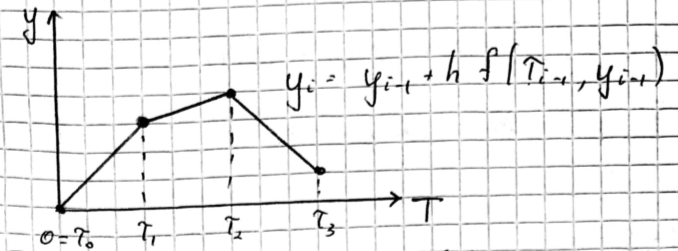
\includegraphics[width=0.5\linewidth]{img/img_19.1}
	\label{img_19.1}
\end{figure}

Покажем, что схема \ref{eq_19_3} аппроксимирует задачу \ref{eq_19_1}. Для этого используем обозначения:

\begin{equation}
\label{eq_19_4}
u_j = y_j + \delta u_j, \;\;\; j = \overline{1, k}
\end{equation}

где ${}^{>}\delta u = [\delta u_0, \delta u_1, ..., \delta u_k > \in {}^{>}\mathbb{R}^{|A_k|}(A_k)$

Для этого рассмотрим схемы:

$$
\begin{cases}
u_0 = u_0\\
\frac{u_i - u_{i - 1}}{h} = f(\tau_{i - 1}, u_{i - 1}), \;\;\; i = \overline{1, k}
\end{cases}
\;\;\;\;\;\;
\begin{cases}
y_0 = u_0\\
\frac{y_i - y_{i-1}}{h} = \frac{y_i(\tau) - y_{i-1}(\tau)}{h}, \;\;\; i = \overline{1, k}
\end{cases}
$$

Используя соотношения \ref{eq_19_4}, отсюда получаем ($u_i - y_i = \delta u_i$)

\begin{equation}
\label{eq_19_5}
\begin{cases}
\delta u_0 = 0\\
\frac{\delta u_i - \delta u_{i - 1}}{h} = f(\tau_{i-1}, y_{i-1} + \delta u_{i-1}) - \frac{y(\tau_i) - y(\tau_i)}{h}
\end{cases}
\end{equation}

где $y(\tau_i) = y(\tau_i) = h y'(\tau_i) + O(h^2) = y(\tau_i) + h(\tau_{i - 1}, y_{i - 1}) + O(h^2), h \to 0$

Отсюда, в соотношениях \ref{eq_19_5}:

\begin{equation}
\label{eq_19_6}
\frac{y(\tau_i) - y(\tau_{i - 1})}{h} = f(\tau_{i - 1}, y_{i - 1}) + O(h), h \to 0
\end{equation}

Поскольку $f$ достаточно гладкая функция, то в \ref{eq_19_5}

\begin{equation}
\label{eq_19_7}
f(\tau_{i - 1}, y_{i - 1} + \delta u_{i - 1}) = f(\tau_{i - 1}, y_{i - 1}) + \frac{\partial f(\tau_{i - 1}, y_{i - 1} + \Theta \delta u_i)}{\partial y}\delta u_{i - 1}
\end{equation}

т.е. $|f(\tau_{i - 1}, y_{i-1}) - f(\tau_{i - 1}, u_{i - 1})| \le M \delta u_{i - 1}, i = \overline{1, k}$, где $M = \left|\left|\frac{\partial f}{\partial y}\right|\right|$

Подставляя \ref{eq_19_6}, \ref{eq_19_7} в \ref{eq_19_5}, получаем:

$$\frac{\delta u_i - \delta u_{i - 1}}{h} = f(\tau_{i - 1}, y_{i - 1} + \delta u_{i - 1}) - f(\tau_{i - 1}, y_{i - 1}) + O(h), h \to 0$$

$$\frac{\delta u_i - \delta u_{i - 1}}{h} = \frac{\partial f(\tau_{i - 1}, y_{i - 1} + \Theta + \delta u_{i - 1})}{\partial y} \cdot \partial u_{i - 1} + O(h), h \to 0$$

Следовательно:

$$
\begin{cases}
|\delta u_i | \le |\delta u_{i - 1}| (1 + hM) + O(h^2), h \to 0\\
i = 1, k
\end{cases}
$$

Отсюда получаем $(1 < j \le k)$:

$$|\delta u_j| \le O(h^2) + (1 + hM) |\delta u_{j - 1}| \le O(h^2) + (1 + hM)(O(h^2) +  (1 - hM)|\delta u_{j - 1}|\le $$
$$\le O(h^2) + (1 + hM) O(h^2) + (1 + hM)^2 O(h^2) + ... + (1 + hM)^{j - 1} O(h^2) + (1 + hM)^j \cdot |\delta u_0| \le $$
$$ \le \{ \text{геом. прогрессия} \} \le \frac{(1 + hM)^k}{(1 + hM) - 1} O(h^2) + (1 + hM)^k |\delta_u| \le e^{Mt} O(h), j = \overline{1, k}$$

так как $\delta u_0 = 0$ и $k = \frac{t}{h} \Rightarrow (1 + hM)^{t/h} \le e^{Mt}; k = h/t \Rightarrow (1 + hM)^{h/t} \le e^M$ 

Таким образом $||{}^{>}\delta u|| = \max \{|\delta u_0|, |\delta u_1|, ..., |\delta u_k|\} \sim O(h), h \to 0$. Следовательно, конечно-разностная схеиа Эйлера \ref{eq_19_3} - корректна и для ломанных Эйлера.

$(spl_1(A_k; {}^{>}u_{(k)}))_{\mathbb{N}}$ следует, что $\lim_{k \to \inf} spl_1(A_k; {}^{>}u_{(k)}) = y$ (равномерная сходимость)
 

\end{document}
